\Askhsh{17805}{2}
\begin{ylh}{1}
    \item 1.3. Πολλαπλασιασμός Αριθμού με Διάνυσμα
    \item 1.4. Συντεταγμένες στο Επίπεδο
    \item 2.3. Εμβαδόν Τριγώνου.
\end{ylh}
\begin{wrapfigure}[17]{r}{0.65\textwidth}
\centering
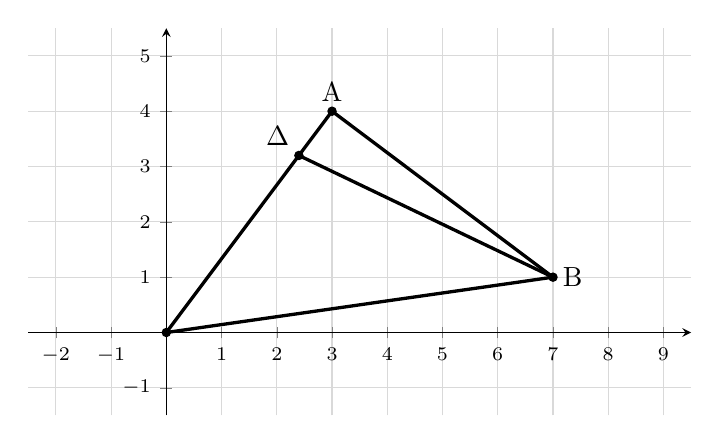
\begin{tikzpicture}
\begin{axis}[
    axis lines = middle,
    xlabel = {},
    ylabel = {},
    xmin = -2.5, xmax = 9.5,
    ymin = -1.5, ymax = 5.5,
    xtick = {-2,-1,0,1,2,3,4,5,6,7,8,9},
    ytick = {-1,0,1,2,3,4,5},
    grid = both,
    grid style = {gray!30},
    width = 10cm,
    height = 6.5cm,
    tick label style = {font=\scriptsize},
    every axis x label/.style = {at={(current axis.right of origin)}, anchor=north west,font=\scriptsize},
    every axis y label/.style = {at={(current axis.above origin)}, anchor=south,font=\scriptsize},
]
    % Draw the segments of triangle OAB
    \addplot[very thick, black] coordinates {(0,0) (3,4)}; % OA
    \addplot[very thick, black] coordinates {(0,0) (7,1)}; % OB
    \addplot[very thick, black] coordinates {(3,4) (7,1)}; % AB

    % Plot points O, A, B, Delta
    \addplot[only marks, mark=*, mark size=1.5pt, black] coordinates {(0,0) (3,4) (7,1) (2.4, 3.2)}; % O, A, B, Delta
    
    % Draw segment Delta B
    \addplot[very thick, black] coordinates {(2.4, 3.2) (7,1)}; % Delta B

    % Labels for points
    \node[above] at (axis cs:3,4) {A};
    \node[right] at (axis cs:7,1) {B};
    \node[above left] at (axis cs:2.4,3.2) {$\Delta$};

\end{axis}
\end{tikzpicture}
\end{wrapfigure}

Δίνεται το τρίγωνο AOB με $A(3,4)$, $B(7,1)$, O η αρχή των αξόνων και το σημείο $\Delta\left(\frac{12}{5}, \frac{16}{5}\right)$ της πλευράς AO.

\begin{alist}
\item Να βρείτε τις συντεταγμένες των διανυσμάτων $\overrightarrow{OA}$ και $\overrightarrow{A\Delta}$. \monades{7}
\item Να δείξετε ότι $\overrightarrow{A\Delta} = -\frac{1}{5}\overrightarrow{OA}$. \monades{9}
\item Δίνεται ότι $(OAB) = \frac{25}{2}$ τετραγωνικές μονάδες. Να δείτε ότι $(A\Delta B) = \frac{1}{5}(OAB)$. \monades{9}
\end{alist}